\documentclass[10pt]{beamer}

\usetheme[progressbar=frametitle]{metropolis}

\usepackage{booktabs}
\usepackage[scale=2]{ccicons}

%used for drawing flow chart
\usepackage{tikz}
\usetikzlibrary{shapes,arrows,positioning,fit,calc}
\usepackage{subfig}

\usepackage{pgfplots}
\usepgfplotslibrary{dateplot}

\usepackage{xspace}
\newcommand{\themename}{\textbf{\textsc{metropolis}}\xspace}

\DeclareMathOperator*{\argmax}{argmax} % no space, limits underneath in displays


\title{Recurrent Human Pose Estimation}
\subtitle{CS 231A Final Project}
\date{\today}
\author{Matthew Chen, Melvin Low}
\institute{Stanford University}
%\titlegraphic{\hfill\includegraphics[height=1.5cm]{logo}}

\begin{document}

\maketitle


\begin{frame}[fragile]{Problem}
Given 2D RGB images with people in them, output a set of coordinates in pixel space corresponding to the joint locations of a single person in the image.

\vspace{10mm}
Motivations
\begin{enumerate}
\item Feature extract for high level learning (activity recognition)
\item Aid inference in robotic / human interaction
\end{enumerate}
\end{frame}

\begin{frame}{Motivation}

\begin{tabular}{l l}
DeepPose (2014)	&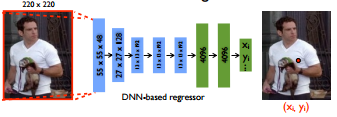
\includegraphics[scale=0.4]{../images/deeppose.png}\\
Pose Machines (2016) &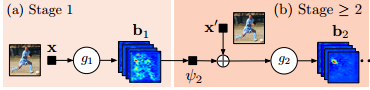
\includegraphics[scale=0.4]{../images/posemachines.png}\\
Stacked Hourglass (2016) &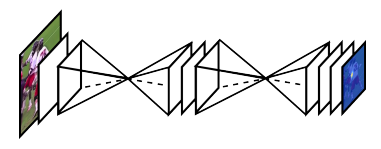
\includegraphics[scale=0.4]{../images/stackedhourglass.png}\\

\end{tabular}

\vspace{10mm}
\textbf{Our Objective}
\begin{align*}
\argmax_{y_i} p(y_i | y_{i-1}, y_{i-2},...,y_1, x), i = 1, 2,...,n
\end{align*}

\end{frame}

\begin{frame}{Methodology}

	%define flowchart elements
\tikzstyle{pipe} = [rectangle, draw, fill=orange!30, rounded corners, text width=4.5em, text height=2em, text badly centered, node distance=7em, inner sep=0pt]
\tikzstyle{line} = [draw, -latex']

\begin{figure}
\begin{center}
\begin{tikzpicture}
\node[pipe] (img) {Image};
\node[pipe, right = 3mm of img] (CNN) {CNN};
\node[pipe, right of=CNN] (lstm3) {LSTM};
\node[pipe, above = 3mm of lstm3] (lstm2) {LSTM};
\node[pipe, above = 3mm of lstm2] (lstm1) {LSTM};

\node[pipe, right = 4mm of lstm1] (head) {Head};
\node[pipe, right = 4mm of lstm2] (sh1) {Shoulder1};
\node[pipe, right = 4mm of lstm3] (sh2) {Shoulder2};


\path[line] (img)--(CNN);
\path[line] (CNN)--(lstm1);
\path[line] (CNN)--(lstm2);
\path[line] (CNN)--(lstm3);
\path[line] (lstm1)--(lstm2);
\path[line] (lstm2)--(lstm3);

\path[line] (lstm1)--(head);
\path[line] (lstm2)--(sh1);
\path[line] (lstm3)--(sh2);
\end{tikzpicture}
\label{model_diag}
\caption{CNN-RNN architecture. A CNN is used to extract features from each image, which are
then fed into an LSTM. The LSTM produces joint coordinates in pixel space.}
\label{fig:lstm_diag}
\end{center}
\end{figure}
\end{frame}

%TODO : Need to modify this to include batch normalization
\begin{frame}{Base Model}
\begin{table}
\tiny
\begin{center}
\begin{tabular}{| c | c | c |}
\hline
Section & Type & Parameters\\
\hline\hline
Layer 1 & conv3-64 & 1,728\\
&conv3-64 & 36,864\\
&maxpool & 0\\
Layer 2&conv3-128 & 73,728\\
&conv3-128 & 147,456\\
&maxpool & 0\\
Layer 3&conv3-256 & 294,912\\
&conv3-256 & 589,824\\
&conv3-256 & 589,824\\
&maxpool & 0\\
Layer 4&conv3-512 & 1,179,648\\
&conv3-512 & 2,359,296\\
&conv3-512 & 2,359,296\\
&maxpool & 0\\
Layer 5&conv3-512 & 2,359,296\\
&conv3-512 & 2,359,296\\
&conv3-512 & 2,359,296\\
&maxpool & 0\\
Layer 6&fc-4096 & 102,760,448\\
Layer 7&fc-4096 & 16,777,216\\
&fc-19 & 77,824\\
&softmax & 0\\
\hline
Total & & 134,325,952\\
\hline
\end{tabular}
\end{center}
\caption{VGGNet architecture and number of parameters}
\label{vgg_arch}
\end{table}
\end{frame}

\begin{frame}{Results}
\begin{figure}
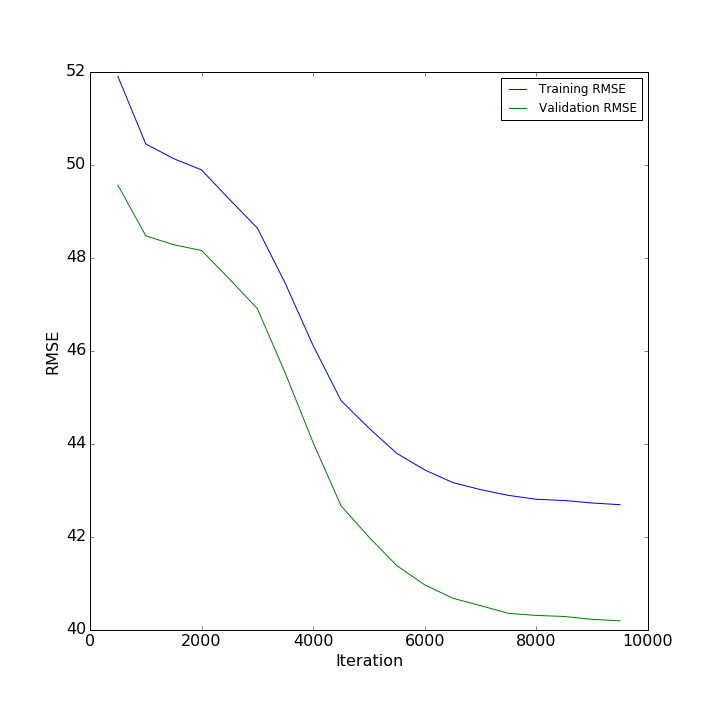
\includegraphics[scale=0.2]{../images/base_loss.png}
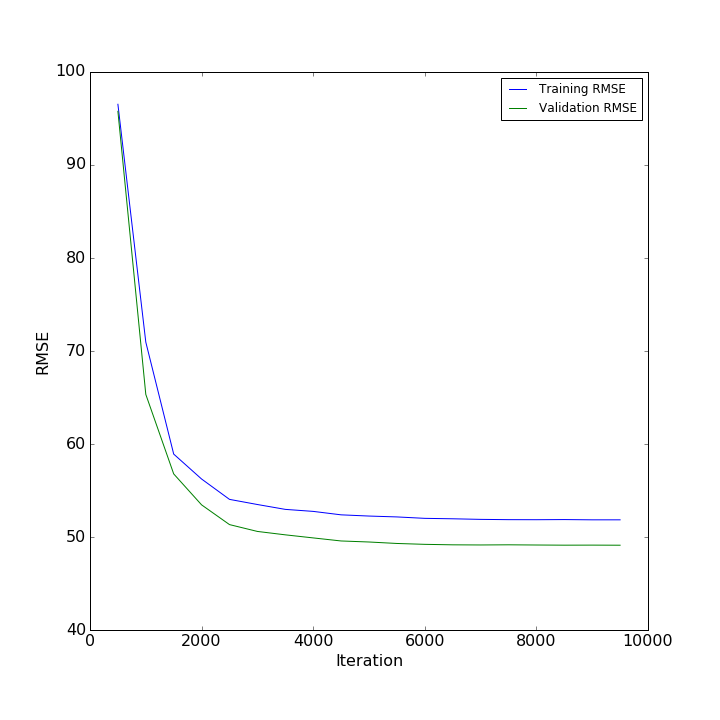
\includegraphics[scale=0.2]{../images/rnn_loss.png}
\caption{Base Model (left) and RNN Model (right)}
\end{figure}
\end{frame}

\begin{frame}{Results - Base Model}
\begin{figure}
\begin{tabular}{cc}
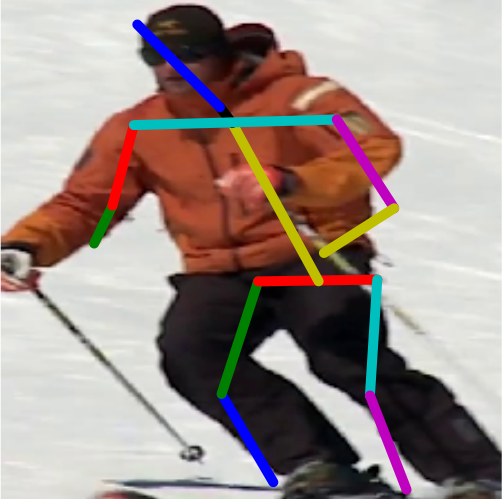
\includegraphics[width=30mm]{../images/base_1}
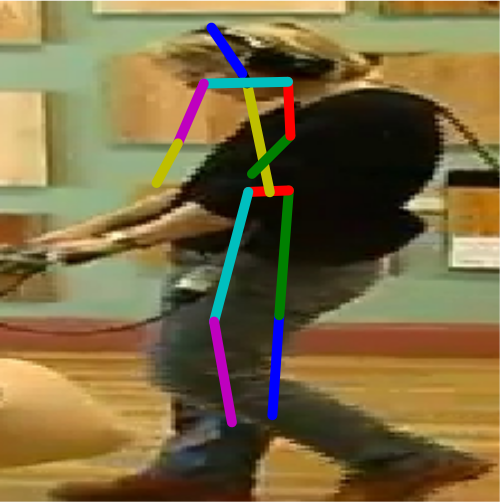
\includegraphics[width=30mm]{../images/base_2}\\
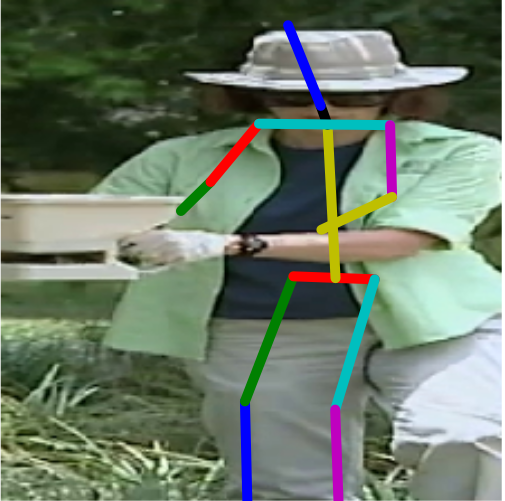
\includegraphics[width=30mm]{../images/base_3}
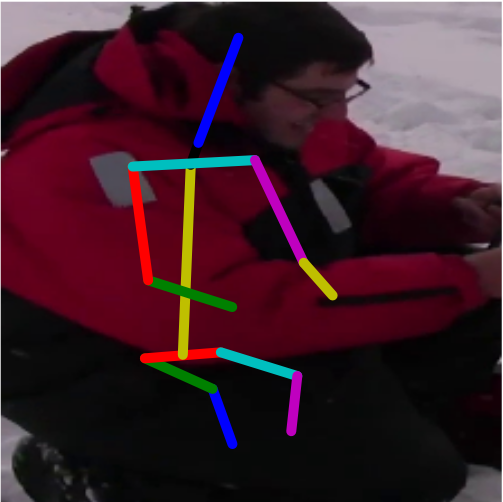
\includegraphics[width=30mm]{../images/base_4}\\
\end{tabular}
\caption{Sample predictions for the CNN base model}
\label{fig:base_images}
\end{figure}
\end{frame}

\begin{frame}{Results - RNN Model}
\begin{figure}
\begin{tabular}{cc}
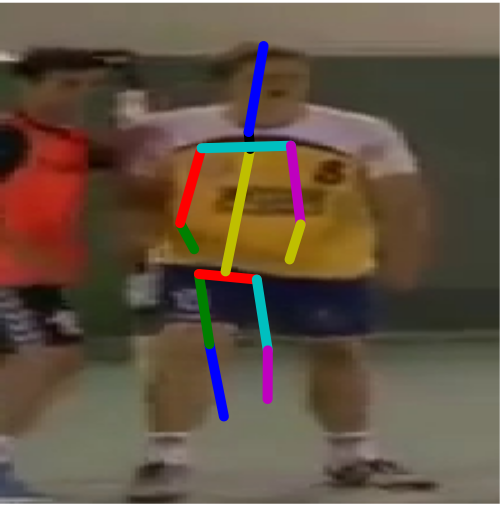
\includegraphics[width=30mm]{../images/rnn_1}
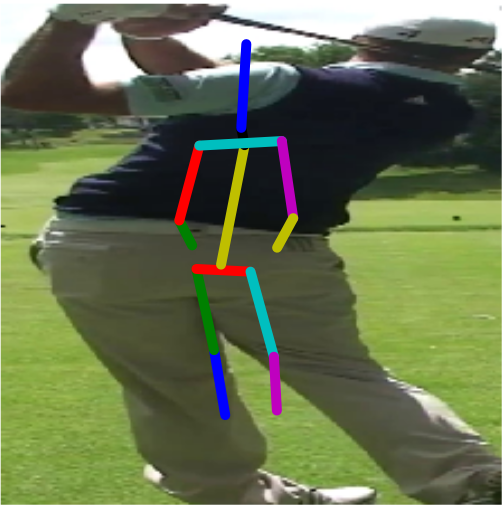
\includegraphics[width=30mm]{../images/rnn_2}\\
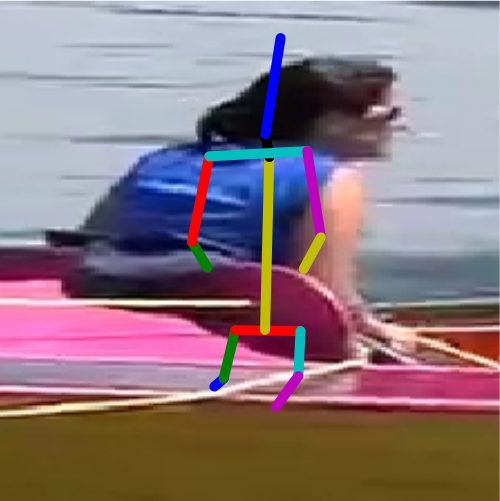
\includegraphics[width=30mm]{../images/rnn_3}
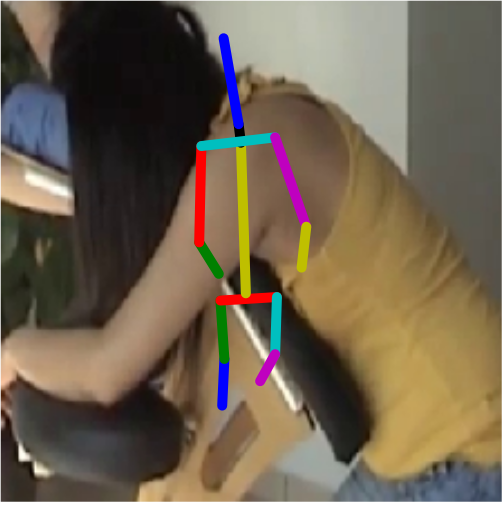
\includegraphics[width=30mm]{../images/rnn_4}\\
\end{tabular}
\caption{Sample predictions for the CNN-RNN model}
\label{fig:rnn_images}
\end{figure}
\end{frame}

\begin{frame}{Conclusion}

\begin{itemize}
\item Qualitative results shown RNN model unable to fit to data
\item Base model outperformed RNN based model
\item Structure likely imposed hard dependencies on joint sequence
\end{itemize}
\end{frame}

\plain{Questions?}

\end{document}
